\section{Interpolation Operator: Discrete Fourier Expansion}
    
    The continuous Fourier series method requires the evaluation of the coefficients
    \begin{align}
        \hat{u}_n = \displaystyle \frac{1}{2\pi} \int_{0}^{2\pi} u(x) e^{-inx} dx.
    \end{align}
    In general, these integrals cannot be computed analytically, and one resorts to the approximation of the Fourier integrals by using quadrature formulas. This procedure defines a discrete transform between the set of values of $u$ at the quadrature points and the set of approximate, or discrete, coefficients. The finite series defined by the discrete transform is actually the interpolate of $u$ at the quadrature nodes. If the properties of accuracy (in particular the spectral accuracy) are retained by replacing the finite transform with the discrete transform, then the interpolant series can be used instead of the truncated series to approximate functions. Also, quadrature formulas differ based on the exact position of the grid points, and the choice of an even or odd number of grid points results in slightly different schemes.
    
    \subsection{The Even Expansion}
    
    Define an equidistant grid, consisting of an even number $N$ of gridpoints $x_j \in [0, 2\pi)$, defined by
	\begin{align*}
        x_j = \frac{2 \pi j}{N} , \hspace{0.5cm} j\in [0, \cdots , N -1]. 
    \end{align*}
    The trapezoidal rule yields the discrete Fourier coefficients $\widetilde{u}_n$, which approximate the continuous Fourier coefficients $\hat{u}_n$ given as follows    
    \begin{align}
        	\widetilde{u}_n = \frac{1}{N}  \displaystyle \sum_{j = 0}^{N - 1} u(x_j) e^{-in x_j}.
    \end{align}
	The difference between the continuous and the discrete approximation is very clear since here we only need precision in the points $ x_j $. This may somehow be an advantage in the numerical calculation because in some cases it is possible to obtain the same order of precision, as shown in the following theorem when trigonometric polynomials are involved, the trapezoidal quadrature rule is a very natural approximation. \\
	
	\begin{teor}
	\label{Exactness_Even}	
	For the points $x_j$ defined as above, the quadrature formula
    \begin{align*}
         \frac{1}{2\pi}\displaystyle \int^{2\pi}_{0} f(x) dx = \frac{1}{N} \displaystyle \sum^{N-1}_{j=0} f(x_j), 
    \end{align*}
    is exact for any trigonometric polynomial $f(x) = e^{inx}$ , $|n| < N$.
    \end{teor}
	\begin{proof}
	Given a function $f(x) = e^{in x}$, It is easy to observe that
	
    \begin{align*}
        \frac{1}{2\pi}\displaystyle \int^{2\pi}_{0} f(x) dx =  \left \lbrace \begin{array}{ll}
    	1 \hspace{3mm} & \text{if } n = 0, \\
    	0 \hspace{3mm} & \text{otherwise.}
    	\end{array}  \right . 
    \end{align*}

	\noindent On the other hand,    
    \begin{align*}
        \frac{1}{N}  \displaystyle \sum_{j = 0}^{N - 1} f(x_j) &= \frac{1}{N}  \displaystyle \sum_{j = 0}^{N - 1} e^{in (\frac{2\pi j}{N})} \\
        &= \frac{1}{N}  \displaystyle \sum_{j = 0}^{N - 1} q^j
    \end{align*}
    where $q = e^{i \frac{2\pi n}{N}}$. If $n$ is an integer multiple of $N$ , i.e., $n = m N$, then, we have to
    \begin{align*}
    	\displaystyle \frac{1}{N} \sum^{N-1}_{j=0}  e^{i Nm (\frac{2\pi j}{N})} = \frac{1}{N} \sum^{N-1}_{j=0}  e^{i(2\pi j m)} = 1
    \end{align*} 
	Otherwise, 
	\begin{align*}
		\displaystyle \frac{1}{N} \sum^{N-1}_{j=0} q^j = \frac{q^{N} - 1}{q - 1} = 0
	\end{align*}
	Thus, the quadrature formula is exact for any function of the form $f(x) = e^{inx}$, $|n| < N$.
	\end{proof}

	Moreover, we can see that the quadrature formula is exact for $f(x) \in \hat{B}_{2N-2}$ where $\hat{B}_N$ is defined as before. Then using the trapezoid rule, the discrete Fourier coefficients become
	\begin{align}
	\label{coeficients_IN}
	    \widetilde{u}_n = \frac{1}{N \widetilde{c}_n}  \displaystyle \sum_{j = 0}^{N - 1} u(x_j) e^{-in x_j},
	\end{align}
	where we introduce the coefficients
	\begin{align}
	\label{constants_IN}	
	    \widetilde{c}_n = \left \lbrace \begin{array}{ll}
	    2  \hspace{0.25cm}\text{if} & |n| =  N/2, \\
	    \\
	    1  \hspace{0.25cm} \text{if} & |n| < N/2.
	\end{array}  \right .
	\end{align}

	\noindent These relations define a new projection of $u$
	\begin{equation}
	\label{collocation_operator_even}
		\mathcal{I}_N u(x) =  \displaystyle \sum_{ |n| \leq \frac {N}{2}} \widetilde{u}_n e^{inx}
	\end{equation}
	This is the complex discrete Fourier transform, based on an even number of quadrature points. From the above, we can see that
	\begin{align*}
	    \widetilde{u}_{-N/2} = \widetilde{u}_{N/2},
	\end{align*}
	so we have exactly $N$ independent Fourier coefficients, corresponding to the $N$ quadrature points. As a consequence, $\mathcal{I}_N \sin( \frac{N}{2} x) = 0$, so that the function $\sin( \frac{N}{2} x)$ is not represented in the above expansion. Therefore, the space $\hat{B}_N$ does not include $\sin( \frac{N}{2} x)$, and the correct space must be as follows
	\begin{align*}
	    \widetilde{B}_N = span\left\{\left(\cos(nx), \hspace{0.2cm} 0 \leq n \leq \frac{N}{2} \right)\cup  \left(\sin(nx), \hspace{0.2cm} 1 \leq n \leq \frac{N}{2} - 1 \right)\right\},
	\end{align*}
	which has dimension dim$(\widetilde{B}_N) = N$.\\
	
	\noindent In the same way, as in the previous subsection using the discrete expansion for Examples \ref{Example1} and \ref{Example2}, we can observe the same behavior as with continuous expansion, but now we have that the error at each point $x_j$ of the grid is zero.

	\begin{example}
	    Consider the $C^{\infty}_p [0, 2 \pi]$ function
    	\begin{align}
    		\label{Example4}
    	    u(x) = \frac{1}{5 - 4 \cos(x)}.
    	\end{align}
    	Its expansion coefficients are
    	\begin{align*}
    	     \hat{u}_{n} = \frac{2^{-|n|}}{3}.
    	\end{align*}
    	\begin{figure}[H]
        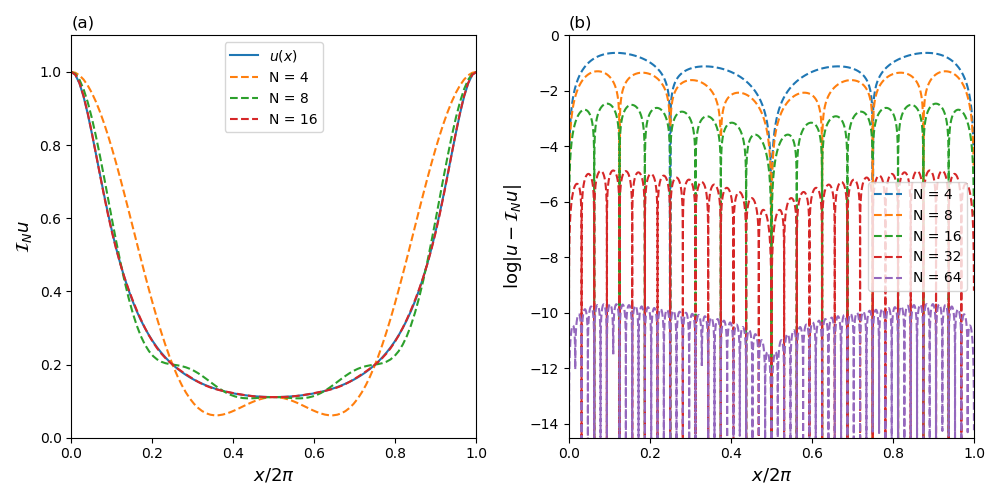
\includegraphics[width=\textwidth]{preliminaries/figures/example23.png}
        \caption{(a) Discrete Fourier series approximation of the equation (\ref{Example4}). (b) Pointwise error of approximation for increasing resolution.}
        \label{fig3}
        \end{figure}
	\end{example} 
	
	\begin{example}
	    The expansion coefficients of the function
    	\begin{align}
    		\label{Example5}
    	    u(x) = \frac{\pi}{2} \sin(\frac{x}{2}),
    	\end{align}
   		are given by
    	\begin{align*}
    	     \hat{u}_{n} = \frac{1}{(1 - 4n^2)}.
    	\end{align*}
    	\begin{figure}[H]
        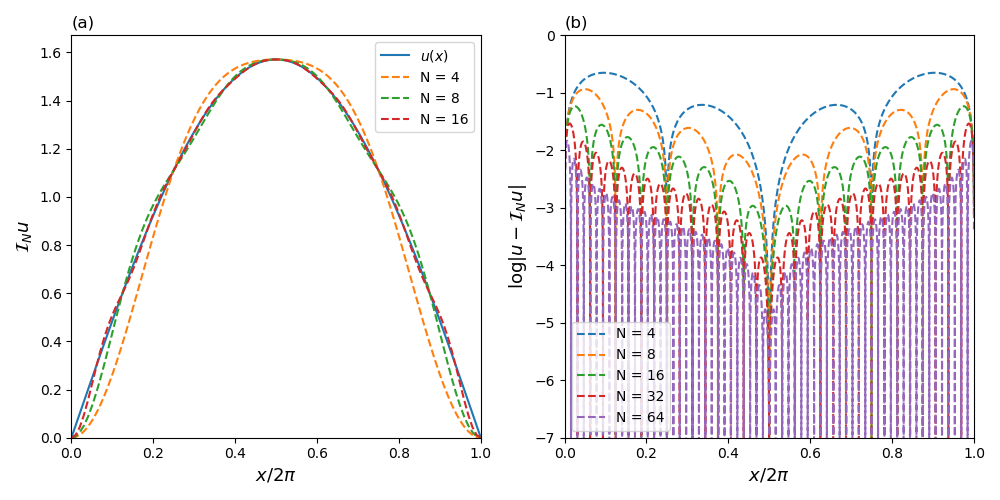
\includegraphics[width=\textwidth]{preliminaries/figures/example24.png}
        \caption{(a) Discrete Fourier series approximation of the equation (\ref{Example5}). (b) Pointwise error of approximation for increasing resolution.}
        \label{fig4}
        \end{figure}
	\end{example} 
	
	Therefore, we can see that the discrete expansion is, in fact, an interpolation operator as mentioned. This can be shown in the following theorem.\\
	
	\begin{teor}
	Let the discrete Fourier transform be defined by Equations (\ref{coeficients_IN})-(\ref{collocation_operator_even}). For any periodic function, $C^{0}_p [0, 2\pi]$, we have
	\begin{align*}
		\mathcal{I}_N u(x_j) = u(x_j), \hspace{0.3cm} \forall x_j = \frac{2 \pi j}{N} , \hspace{0.3cm} j = 0, \dots, N - 1. 
	\end{align*}
	\end{teor}

	\begin{proof}
	Substituting Equation (\ref{coeficients_IN}) into Equation (\ref{collocation_operator_even}) we obtain
	
	\begin{equation*}
    	\mathcal{I}_N u(x) =  \displaystyle \sum_{ |n| \leq \frac {N}{2}} \left(\frac{1}{N \widetilde{c}_n}  \displaystyle \sum_{j = 0}^{N - 1} u(x_j) e^{-in x_j}\right) e^{inx}.
	\end{equation*}
	Exchanging the order of the sum gives
	\begin{align}
	    \mathcal{I}_N u(x) = \displaystyle \sum_{j=0}^{N-1} u(x_j) g_j (x),
	\end{align}
	where
	\begin{align*}
	    g_j (x) &= \displaystyle \sum_{ |n| \leq \frac {N}{2}} \frac{1}{N \widetilde{c}_n} e^{in(x -x_j)}\\
	    &= \frac{1}{N} \sin\left[N \frac{x - x_j}{2} \right] \cot\left[\frac{x - x_j}{2} \right]
	\end{align*}
	by summing as a geometric series. It is easily verified that $g_j (x_i) = \delta_{ij}$\\
	\\
	We still need to show that $g_j (x) \in \widetilde{B}_N$. Clearly, $g_j (x) \in \hat{B}_N$ as $g_j (x)$ is a polynomial of degree $\leq N/2$. However, since
	
	\begin{align*}
	    \frac{1}{2} e^{-i \frac{N}{2} x_j} = \frac{1}{2} e^{i \frac{N}{2} x_j} = \frac{(-1)^j}{2},
	\end{align*}
	
	and, by convention $\widetilde{u}_{-N/2} = \widetilde{u}_{N/2}$, we do not get any contribution from the term $\sin(\frac{N}{2} x)$, hence $g_j (x) \in \widetilde{B}_N$.
	\end{proof}
	
	\subsection{The Odd Expansion}
	
	Similarly, we define a grid with an odd number of grid points as follows
	\begin{align*}
        x_j = \frac{2 \pi}{N + 1} j , \hspace{0.5cm} j\in [0, \dots , N],
    \end{align*}
    and using the trapezoidal rule we get
	\begin{align}
	\label{coefficients_JN}
        \widetilde{u}_n = \frac{1}{N + 1}  \displaystyle \sum_{j = 0}^{N} u(x_j) e^{-in x_j},
    \end{align}
    to obtain the interpolation operator
    \begin{equation}
    \label{Interpolation_operator_odd}
    	\mathcal{J}_N u(x) =  \displaystyle \sum_{ |n| \leq \frac {N}{2}} \widetilde{u}_n e^{inx}.
	\end{equation}
	
    \noindent Again as before, the quadrature formula is highly accurate. \\
    \begin{teor}
    \label{Exactness_Odd}	
    For the points $x_j$ defined as above, the quadrature formula
    \begin{align*}
         \frac{1}{2\pi}\displaystyle \int^{2\pi}_{0} f(x) dx = \frac{1}{N+1} \displaystyle \sum^{N}_{j=0} f(x_j),
    \end{align*}
    is exact for any $f(x) = e^{inx}$ , $|n| < N$, i.e., for all $f(x) \in \widetilde{B}_{2N}$.
    \begin{proof}
    	Given a function $f(x) = e^{in x}$, It is easy to observe that
    	
    	\begin{align*}
    		\frac{1}{2\pi}\displaystyle \int^{2\pi}_{0} f(x) dx =  \left \lbrace \begin{array}{ll}
    			1 \hspace{3mm} & \text{if } n = 0, \\
    			0 \hspace{3mm} & \text{otherwise.}
    		\end{array}  \right . 
    	\end{align*}
    	On the other hand,    
    	\begin{align*}
    		\frac{1}{N+1}  \displaystyle \sum_{j = 0}^{N} f(x_j) &= \frac{1}{N+1}  \displaystyle \sum_{j = 0}^{N} e^{in (\frac{2\pi j}{N+1})} \\
    		&= \frac{1}{N+1}  \displaystyle \sum_{j = 0}^{N} q^j
    	\end{align*}
    	where $q = e^{i \frac{2\pi n}{N+1}}$. If $n$ is an integer multiple of $N+1$ , i.e., $n = (N+1)m$, then we have to
    	\begin{align*}
    		\displaystyle \frac{1}{N+1} \sum^{N}_{j=0}  e^{i(N+1)m (\frac{2\pi j}{N+1})} = \frac{1}{N+1} \sum^{N}_{j=0}  e^{i (2\pi jm)} = 1
    	\end{align*}
    	 Otherwise, 
    	\begin{align*}
    		\displaystyle \frac{1}{N+1} \sum^{N}_{j=0} q^j = \frac{q^{N+1} - 1}{q - 1} = 0
    	\end{align*}
    	Thus, the quadrature formula is exact for any function of the form $f(x) = e^{inx}$, $|n| < N$.
    \end{proof}
    
    \end{teor}
    The scheme may also be expressed through the use of a Lagrange interpolation polynomial,
    \begin{align}
    \label{Lagrange_Odd}	
    	\mathcal{J}_N u(x) =  \displaystyle \sum_{j=0}^{N} u(x_j) h_j (x)
	\end{align}
	where
	\begin{align}
	    h_j (x) = \displaystyle \frac{1}{N+1} \sum_{|k| \leq \frac{N}{2}} e^{ik (x - x_j)} = \frac{1}{N + 1} \frac{\sin(\frac{N+1}{2}(x - x_j))}{\sin(\frac{x - x_j}{2})}
	\end{align}
    One easily shows that $h_j (x_l) = \delta_{jl}$ and that $h_j (x) \in \hat{B}_N $.
	
	\newpage
    \subsection{Differentiation of the discrete expansions}
    
    Similarly, as in continuous expansion, we require compute derivatives of the discrete approximation. In the following subsections, we assume that our function $u$ and all its derivatives are continuous and periodic on $[0, 2\pi]$.\\
    \\
    We consider the case of an even number of grid points. Using expansion coefficients given the values of the function $u(x)$ at the points $x_j$ , differentiating the basis functions in the interpolant yields
    \begin{align}
        \frac{d}{dx} \mathcal{I}_N u(x) = \displaystyle \sum_{|n| \leq N/2} in \widetilde{u}_n e^{inx}, \hspace{2mm} \widetilde{u}_n = \displaystyle \frac{1}{N \widetilde{c}_n} \sum_{j=0}^{N-1} u(x_j) e^{-in x_j},   
    \end{align}
    where $\widetilde{c}_n$ is given by (\ref{constants_IN}). Higher order derivatives can be obtained simply by further differentiating the basis functions.\\
    
    \noindent Similarly, for the case of an odd number of grid points
    \begin{align}
    	\frac{d}{dx} \mathcal{J}_N u(x) = \displaystyle \sum_{|n| \leq N/2} in \widetilde{u}_n e^{inx}, \hspace{2mm} \widetilde{u}_n = \displaystyle \frac{1}{N + 1} \sum_{j=0}^{N} u(x_j) e^{-in x_j},   
    \end{align} 
    The procedure for differentiating using expansion coefficients can be described as follows: first, we transform the point values $u(x_j)$ in physical space into the coefficients $\widetilde{u}_n$ in mode space. We then differentiate in mode space by multiplying  $\widetilde{u}_n$ by $in$, and return to physical space.\\
    
    There are other ways to obtain these derivatives, which may have greater advantage and be more efficient to calculate. In the literature, it can commonly find the use of differentiation matrices, for which there is a great variety. We will present some matrices that have been studied in \cite{gottlieb2007}, \cite{Canuto2012}, and we will observe the difference between the cases of an even and odd number of grid points. \\
    
    \paragraph{Differentiation Matrix.} Recall that to the case of an even number of grid points, the interpolation operator can be written as
    \begin{align*}
        \mathcal{I}_N u(x) = \displaystyle \sum^{N-1}_{j=0} u(x_j) g_j (x),
    \end{align*}
    where $g_j$ are the Lagrange interpolation polynomials given by
    \begin{align*}
        g_j (x) = \frac{1}{N} \sin\left[N \frac{x - x_j}{2} \right] \cot\left[\frac{x - x_j}{2} \right].
    \end{align*}
    Then, by differentiating the interpolation directly, it can get an approximation to the derivative of $u(x)$ at the points $x_j$ as follows
    \begin{align*}
        \displaystyle \frac{d}{dx} \mathcal{I}_N (x) \Big|_{x_l} = \sum^{N-1}_{j=0} u(x_j) \frac{d}{dx} g_j (x) \Big|_{x_l} = \sum^{N-1}_{j=0} D_{lj} u(x_j),
    \end{align*}
    where $D_{lj}$ are the differentiation matrix entries given by
    \begin{align}
    \label{matrix_DN_even}
        D_{ij} = \frac{d}{dx} g_j (x) \Big|_{x_i} = \begin{cases} \frac{(-1)^{i+j}}{2} \cot \left[ \frac{x_i - x_j}{2}\right] &   i \neq j, \\ \hspace{1mm} 0 &  i=j, \end{cases}
    \end{align}
    it is also well known that $D$ is circulant and skew-symmetric matrix. In the same way, the entries of the second order differentiation matrix $D^{(2)}$ gives us
    \begin{align}
    \label{matrix_D2N_even}
        D_{ij}^{(2)} = \frac{d^2}{dx^2} g_j (x) \Big|_{x_i} = \begin{cases} -\frac{(-1)^{i+j}}{2} \left[\sin \left[ \frac{x_i - x_j}{2}\right]\right]^{-1} &   i \neq j, \\ -\frac{N^2 + 2}{12} &  i=j. \end{cases}
    \end{align}
	
    The approximation of higher derivatives follows exactly the same route, and similarly to obtain the entries of the differentiation matrix $\widetilde{D}$ for the interpolation based on an odd number of points given by
    \begin{align}
    \label{matrix_DN_odd}
        \widetilde{D}_{ij} = \begin{cases} -\frac{(-1)^{i+j}}{2} \left[\sin \left[ \frac{x_i - x_j}{2}\right]\right]^{-2} &   i \neq j, \\ \hspace{1mm} 0 &  i=j. \end{cases}
    \end{align}

    It is also known that $\widetilde{D}$ is a circulant, skew-symmetric matrix. The advantage of this method is that the differentiation matrix takes us from physical space to physical space, and the act of differentiation is hidden in the matrix itself. \\
    
    It is interesting to observe that the differentiation operator for the interpolation based on an odd number of grid points, takes elements of $\widetilde{B}_N$ out of $\widetilde{B}_N$ and then
    \begin{align*}
    	\mathcal{I}_N \frac{d^2}{dx^2} \mathcal{I}_N \neq \left( \mathcal{I}_N \frac{d}{dx} \right)^2 \mathcal{I}_N.
    \end{align*}
	
	But for the interpolation based on an odd number of grid points the differentiation operator remain in $\hat{B}_N$ when takes elements of $\hat{B}_N$, and thus,
	\begin{align*}
		\mathcal{J}_N \frac{d^2}{dx^2} \mathcal{J}_N = \left( \mathcal{J}_N \frac{d}{dx} \right)^2 \mathcal{J}_N
	\end{align*}
    Moreover, for all values of $q$ we have
    \begin{align*}
        \widetilde{D}^{(q)} = \mathcal{J}_N \frac{d^q}{dx^q} \mathcal{J}_N = \widetilde{D}^q
    \end{align*}
	allowing us to calculate approximate high derivatives by just multiplying the $D$ matrix as many times as necessary.
    
    For the above, and for some interesting properties that we will see later about interpolation operator based on an odd number of grid points, it has been decided to use it for the study of this work.
    
    \subsection{Approximation theory for Discrete Expansion.}
    
    Based on the theory developed in \cite{gottlieb2007} with respect to the interpolation operator analysis for the case of an even number of grid points, we will adapt the results for the case of an odd number of grid points in the most detailed way possible. \\
    
    \noindent First of all, we can define a discrete version of the inner product $L^2$ as follows
    \begin{align*}
    	\langle f_N, g_N \rangle_N = \displaystyle \frac{1}{N + 1} \sum_{j = 0}^{N} f_N (x_j) \bar{g}_N (x_j),
    \end{align*}
	and the associated norm
	\begin{align*}
		\| f_N \|_N^2 = \langle f_N, f_N \rangle_N
	\end{align*}
	where $f_N$ , $g_N \in \hat{B}_N$ and there are an odd number of grid points $x_j$ , $j = 0, \dots , N$. Note also that the interpolant $\mathcal{J}_N u$ of a continuous function $u$ and for all $v \in \hat{B}_N$, satisfies trivially the identity
	\begin{align*}
		\langle \mathcal{J}_N u, v \rangle_N = \langle u, v \rangle_N.
	\end{align*} 
	
	Moreover, as a consequence of the exactness of the quadrature rule for trigonometric functions, as have seen in Theorem \ref{Exactness_Even}, we have
	\begin{align}
	\label{Coincidence_Inner}	
		\langle f_N, g_N \rangle_N = \displaystyle \frac{1}{2 \pi} \int_{0}^{2 \pi} f_N \bar{g}_N dx, \hspace{3mm} \|f_N\|_{L^2 [0, 2 \pi]} = \|f_N\|_N
	\end{align}

	Hence, in $\hat{B}_N$ , the continuous and discrete inner product are the same.\\
	
	The situation is different when we discuss an even number of grid points. If $f_N , g_N \in \tilde{B}_N$ and we have an even number of grid points $x_j$ , the discrete inner product
	\begin{align*}
		\langle f_N, g_N \rangle_N = \displaystyle \frac{1}{N} \sum_{j = 0}^{N - 1} f_N (x_j) \bar{g}_N (x_j), \hspace{3mm} \|f_N\|_N^2 = \langle f_N, f_N \rangle_N
	\end{align*}
	is not equal to the continuous inner product. However, using the fact that $f_N \in L^2 [0, 2 \pi]$ it can be shown that there exists a $K > 0$ such that
	\begin{align}
	\label{equivalent_discrete_continous}
		K^{-1} \|f_N\|^2_{L^2 [0, 2 \pi]} \leq \|f_N\|^2_N \leq K \|f_N\|^2_{L^2 [0, 2 \pi]}.
	\end{align}
    
    Something very interesting and useful in the use of discrete expansion to approximate functions and their derivatives is that the behavior is very similar to that shown in the previous subsection for continuous expansion. We will see that the approximation theory for the discrete expansion yields essentially the same results as for the continuous expansion. The proofs are based on the fact that the Fourier coefficients of the discrete approximation are sufficiently close to those of the continuous approximation. \\
    
    Recall that the interpolation operator associated with an odd number of grid points is given by
    \begin{align*}
    	\mathcal{J}_{2N} u = \displaystyle \sum_{|n|\leq N} \widetilde{u}_n e^{inx},
    \end{align*}
    with expansion coefficients
    \begin{align*}
    	\widetilde{u}_n = \displaystyle \frac{1}{2N + 1} \sum^{2N}_{j=0} u(x_j)e^{-in x_j}, \hspace{2mm} x_j = \frac{2 \pi j}{2N+1}.
    \end{align*}
    
    First we observe the following, the interpolation operator associated with an odd number of grid points are based on the points $x_j$, for which the $(n + Mm)$th mode, where $M = 2N + 1$, is indistinguishable from  the $n$th mode, i.e.,
    \begin{align*}
    	e^{i(n + Mm)x_j} = e^{in x_j} e^{i 2 \pi m j} = e^{in x_j}
    \end{align*}
	This phenomenon is known as aliasing.\\
	
	Moreover, due to the orthogonality relation as before seen we have to
    \begin{align*}
    	\frac{1}{M} \displaystyle \sum^{M-1}_{j=0} e^{-inx_j} =  \left \lbrace \begin{array}{ll}
    	1 \hspace{4mm} &\text{if} \hspace{2mm} n=M m, \hspace{2mm} m = 0, \pm 1, \pm 2, \dots, \\
    	0 &\text{otherwise.}
    	\end{array}  \right .
    \end{align*} 
    
    The relationship between the discrete expansion coefficients $\widetilde{u}_n$ , and the continuous expansion coefficients $\hat{u}_n$, is given in the following lemma. 
    
    \begin{lemma}
    \label{lemma_2.1}
    Consider $u(x) \in W^q_p [0, 2\pi]$, where $q > 1/2$. For $|n| \leq N$ we have
	    \begin{align}
	    \label{alias}   
	        \widetilde{c}_n \widetilde{u}_n = \displaystyle \hat{u}_n + \sum_{\substack{|m|\leq \infty \\ m \neq 0}} \hat{u}_{n + Mm}
	    \end{align}
	\end{lemma}
	\begin{proof}
    Substituting the continuous Fourier expansion into the discrete expansion yields
    \begin{align*}
        \widetilde{c}_n \widetilde{u}_n = \frac{1}{M} \displaystyle \sum_{j=0}^{M - 1} \sum_{|l| \leq \infty} \hat{u}_l e^{i(l -n)x_j}
    \end{align*}
    To interchange the two summations we must ensure uniform convergence, i.e., $\sum_{|l| \leq \infty} |\hat{u}_l| < \infty$. This is satisfied, since if $q> 1/2$ then, as before there is $m \in \mathbb{N}$ such that for $l \geq m$ we have to
    \begin{align*}
    	(1 + |l|)^{2q} \leq 2q(1 + l^{2q}) 
    \end{align*}
	taking $m$ as follows 
	\begin{align*}
		\frac{1}{m} \leq (2q)^{\frac{1}{2q}} - 1 
	\end{align*}

	\noindent Therefore
    \begin{align*}
        \displaystyle \sum_{|l| \leq \infty} |\hat{u}_l| &= \sum_{|l| \leq \infty} (1 + |l|)^q \frac{|\hat{u}_l|}{(1 + |l|)^q}  \\
        &\leq \left( 2q \sum_{|l| \leq \infty}  (1 + l^{2q}) |\hat{u}_l|^2 \right)^{1/2} \left(\sum_{|l| \leq \infty} (1 + |l|)^{-2q}  \right)^{1/2},
    \end{align*}
    where the last expression follows from the Cauchy-Schwarz inequality. As $u(x) \in W^q_p [0, 2\pi]$ the first part is clearly bounded. Furthermore, the second term is a $p$-series and then converges provided $q > 1/2$, ensuring boundedness. \\
    
    Interchanging the order of summation and using orthogonality of the exponential function at the grid yields the desired result
    \begin{align*}
    	\widetilde{c}_n \widetilde{u}_n &= \frac{1}{M} \displaystyle \sum_{j=0}^{M - 1} \sum_{|l| \leq \infty} \hat{u}_l e^{i(l -n)x_j} =  \sum_{|l| \leq \infty} \frac{1}{M} \sum_{j=0}^{M - 1} \hat{u}_l e^{i(l -n)x_j} \\
    	&= \sum_{|m| \leq \infty}  \frac{1}{M} \sum_{j=0}^{M - 1} \hat{u}_{n + Mm} e^{i(n + Mm)x_j} \\
    	&= \frac{1}{M} \sum_{j=0}^{M - 1} \hat{u}_n e^{inx_j}
    	+ \sum_{\substack{|m|\leq \infty \\ m \neq 0}} \frac{1}{M} \sum_{j=0}^{M - 1} \hat{u}_{n + Mm} e^{i(n + Mm)x_j} \\
    	&= \hat{u}_n + \sum_{\substack{|m|\leq \infty \\ m \neq 0}} \hat{u}_{n + Mm}
    \end{align*}
	\end{proof}
	
	The conclusions of the previous discussion are equally valid in the number of odd or even points. An equivalent formulation of (\ref{alias}) is
	\begin{align*}
		\mathcal{J}_N u = \mathcal{P}_N u + \mathcal{A}_N u
	\end{align*}
	It is orthogonal to the truncation error, $u - \mathcal{P}_N u$, so that
	\begin{align*}
		\| u - \mathcal{J}_N u \|^2 = \|u - P_N u \|^2 + \| \mathcal{A}_N u \|^2
	\end{align*}
	Hence, the error due to the interpolation is actually always larger than the error due to the truncation of the Fourier series.\\
	
	Rather than deriving the estimates of the approximation error directly, we shall use the results obtained in the previous section and then estimate the difference between the two different expansions, which we recognize as the aliasing error given by
	\begin{align*}
		\| \mathcal{A}_N \|_{L^2 [0, 2\pi]} = \left\| \displaystyle \sum_{|n|<N} \left( \sum_{\substack{|m|\leq \infty \\ m \neq 0}} \hat{u}_{n + Mm}  \right) \right\|_{L^2 [0, 2\pi]}
	\end{align*}
    
    As before, we first consider the behavior of the approximation in the $L^2$-norm. We will first show that the bound on the aliasing error, $\mathcal{A}_N$ , in equation above is of the same order as the truncation error. The error caused by truncating the continuous expansion is essentially the same as the error produced by using the discrete coefficients rather than the continuous coefficients.
    \begin{lemma}
    \label{estimating_aliasing_error}	
    For any $u(x) \in W_p^r [0, 2\pi]$, where $r > 1/2$, the aliasing error
    \begin{align*}
        \| \mathcal{A}_N \|_{L^2 [0, 2\pi]} = \displaystyle \left(\sum_{|n| \leq \infty} |\widetilde{c}_n \widetilde{u}_n - \hat{u}_n|^2 \right)^{1/2} \leq CN^{-r} \|u^{r}\|_{L^2 [0, 2\pi]}
    \end{align*}
	\end{lemma}
	\begin{proof}
    From Lemma \ref{lemma_2.1} we have
    \begin{align*}
        |\widetilde{c}_n \widetilde{u}_n - \hat{u}_n|^2 = \displaystyle \left|\sum_{\substack{|m|\leq \infty \\ m \neq 0}} \hat{u}_{n + Mm} \right|^2
    \end{align*}
    To estimate this, we first note that
    \begin{align*}
        \displaystyle \left|\sum_{\substack{|m|\leq \infty \\ m \neq 0}} \hat{u}_{n + Mm} \right|^2 &= \left|\sum_{\substack{|m|\leq \infty \\ m \neq 0}} |n + Mm|^r \hat{u}_{n + Mm} \frac{1}{|n + Mm|^r} \right|^2 \\ 
        &\leq \left(\sum_{\substack{|m|\leq \infty \\ m \neq 0}} |n + Mm|^{2r} |\hat{u}_{n + Mm}|^2 \right) \left(\sum_{\substack{|m|\leq \infty \\ m \neq 0}} \frac{1}{|n + Mm|^{2r}}  \right)
    \end{align*}
    using the Cauchy-Schwartz inequality. Since $M =2N + 1$ and  $|n| \leq N$, we have to $N(2m - 1) = 2Nm - N \leq |n + Mm|$. Hence, bounding of the second term is ensured by
    \begin{align*}
        \displaystyle \sum_{\substack{|m|\leq \infty \\ m \neq 0}} \frac{1}{|n + Mm|^{2r}} \leq \frac{2}{N^{2r}} \sum^{\infty}_{m=1} \frac{1}{(2m - 1)^{2r}} = C_1 N^{-2r},
    \end{align*}
    provided $r > 1/2$. Here, the constant $C_1$ is a consequence of the fact that the power series converges, and it is independent of $N$.\\
    Summing over $n$, we have
    \begin{align*}
        \displaystyle \sum_{|n|\leq N} \left|\sum_{\substack{|m|\leq \infty \\ m \neq 0}} \hat{u}_{n + Mm} \right|^2 &\leq \sum_{|n| \leq N} C_1 N^{-2r} \sum_{\substack{|m|\leq \infty \\ m \neq 0}} |n + Mm|^{2r} |\hat{u}_{n + Mm}|^2 \\
        &\leq C_2 N^{-2r} \| u^{(r)} \|^2_{L^2[0, 2\pi]}
    \end{align*}
	\end{proof}

    We are now in a position to state the error estimate for the discrete approximation.
    \begin{teor}
    \label{estimating_error_I_N_L2}	
    For any $u(x) \in W_p^r [0, 2\pi]$ with $r > 1/2$, there exists a positive constant $C$, independent of $N$ , such that
    \begin{align*}
        \| u - \mathcal{J}_{2N}u \|_{L^2 [0, 2\pi]} \leq CN^{-r} \| u^{(r)} \|_{L^2 [0, 2\pi]}
    \end{align*}
	\end{teor}
    \begin{proof}
    Let’s write the difference between the function and its discrete approximation
    \begin{align*}
        \| u - \mathcal{J}_{2N}u \|_{L^2 [0, 2\pi]} &= \| (\mathcal{P}_{2N} - \mathcal{J}_{2N})u + u - \mathcal{P}_{2N}u \|_{L^2 [0, 2\pi] } \\
        &\leq  \| (\mathcal{P}_{2N} - \mathcal{J}_{2N})u \|_{L^2 [0, 2\pi] } + \| u - \mathcal{P}_{2N}u \|_{L^2 [0, 2\pi] }
    \end{align*}
    Thus, the error has two components. The first one, which is the difference between the continuous and discrete expansion coefficients, is the aliasing error, which is bounded in Lemma \ref{estimating_aliasing_error}. The second, which is the tail of the series, is the truncation error, which is bounded by the result of Theorem \ref{estimating_error_PN_L2}. The desired result follows from these error bounds.
	\end{proof}

    Theorem above confirms that the approximation errors of the continuous expansion and the discrete expansion are of the same order, as long as $u(x)$ has at least half a derivative. Furthermore, the rate of convergence depends, in both cases, only on the smoothness of the function being approximated.   